\documentclass[12pt,titlepage]{article}

\setlength{\oddsidemargin}{0in}
\setlength{\evensidemargin}{0in}
\setlength{\textwidth}{6.5in}
%
\setlength{\textheight}{9in}
\setlength{\topmargin}{0in}
\setlength{\headsep}{0in}
\setlength{\topskip}{0in}
\setlength{\headheight}{0in}

\usepackage{graphicx}
\usepackage{times}
\usepackage[plainpages=false, colorlinks=true, anchorcolor=blue, linkcolor=blue, citecolor=blue, bookmarks=false, urlcolor=blue]
{hyperref}
\usepackage[square,comma,authoryear]{natbib}


\title{DOE Office of Science INCITE Project:\\
{\it Extreme-scale Simulation of Supernovae and Magnetars from Realistic Progenitors}\\
2019 EOY Report}

\author{Principal Investigator:\\Sean M. Couch\\
  Michigan State University \vspace{0.1in}\\
  Co-Investigators: \\
  Andrew Christlieb (Michigan State University) \\
  Evan O'Connor (Stockholm University)\\
  Kuo-Chuan Pan (National Tsinghua University) \\
  Luke Roberts (Michigan State University) \\
  MacKenzie Warren (North Carolina State University) \\
}

\date{January 1, 2020}


\begin{document}


\maketitle


%%%%%%%%%%%%%%%%%%%%%%%%%%%%%%%%%
\section{Project Usage}

%%%%%%%%%%%%%%%%%%%


\begin{figure}
  \begin{tabular}{cc}
    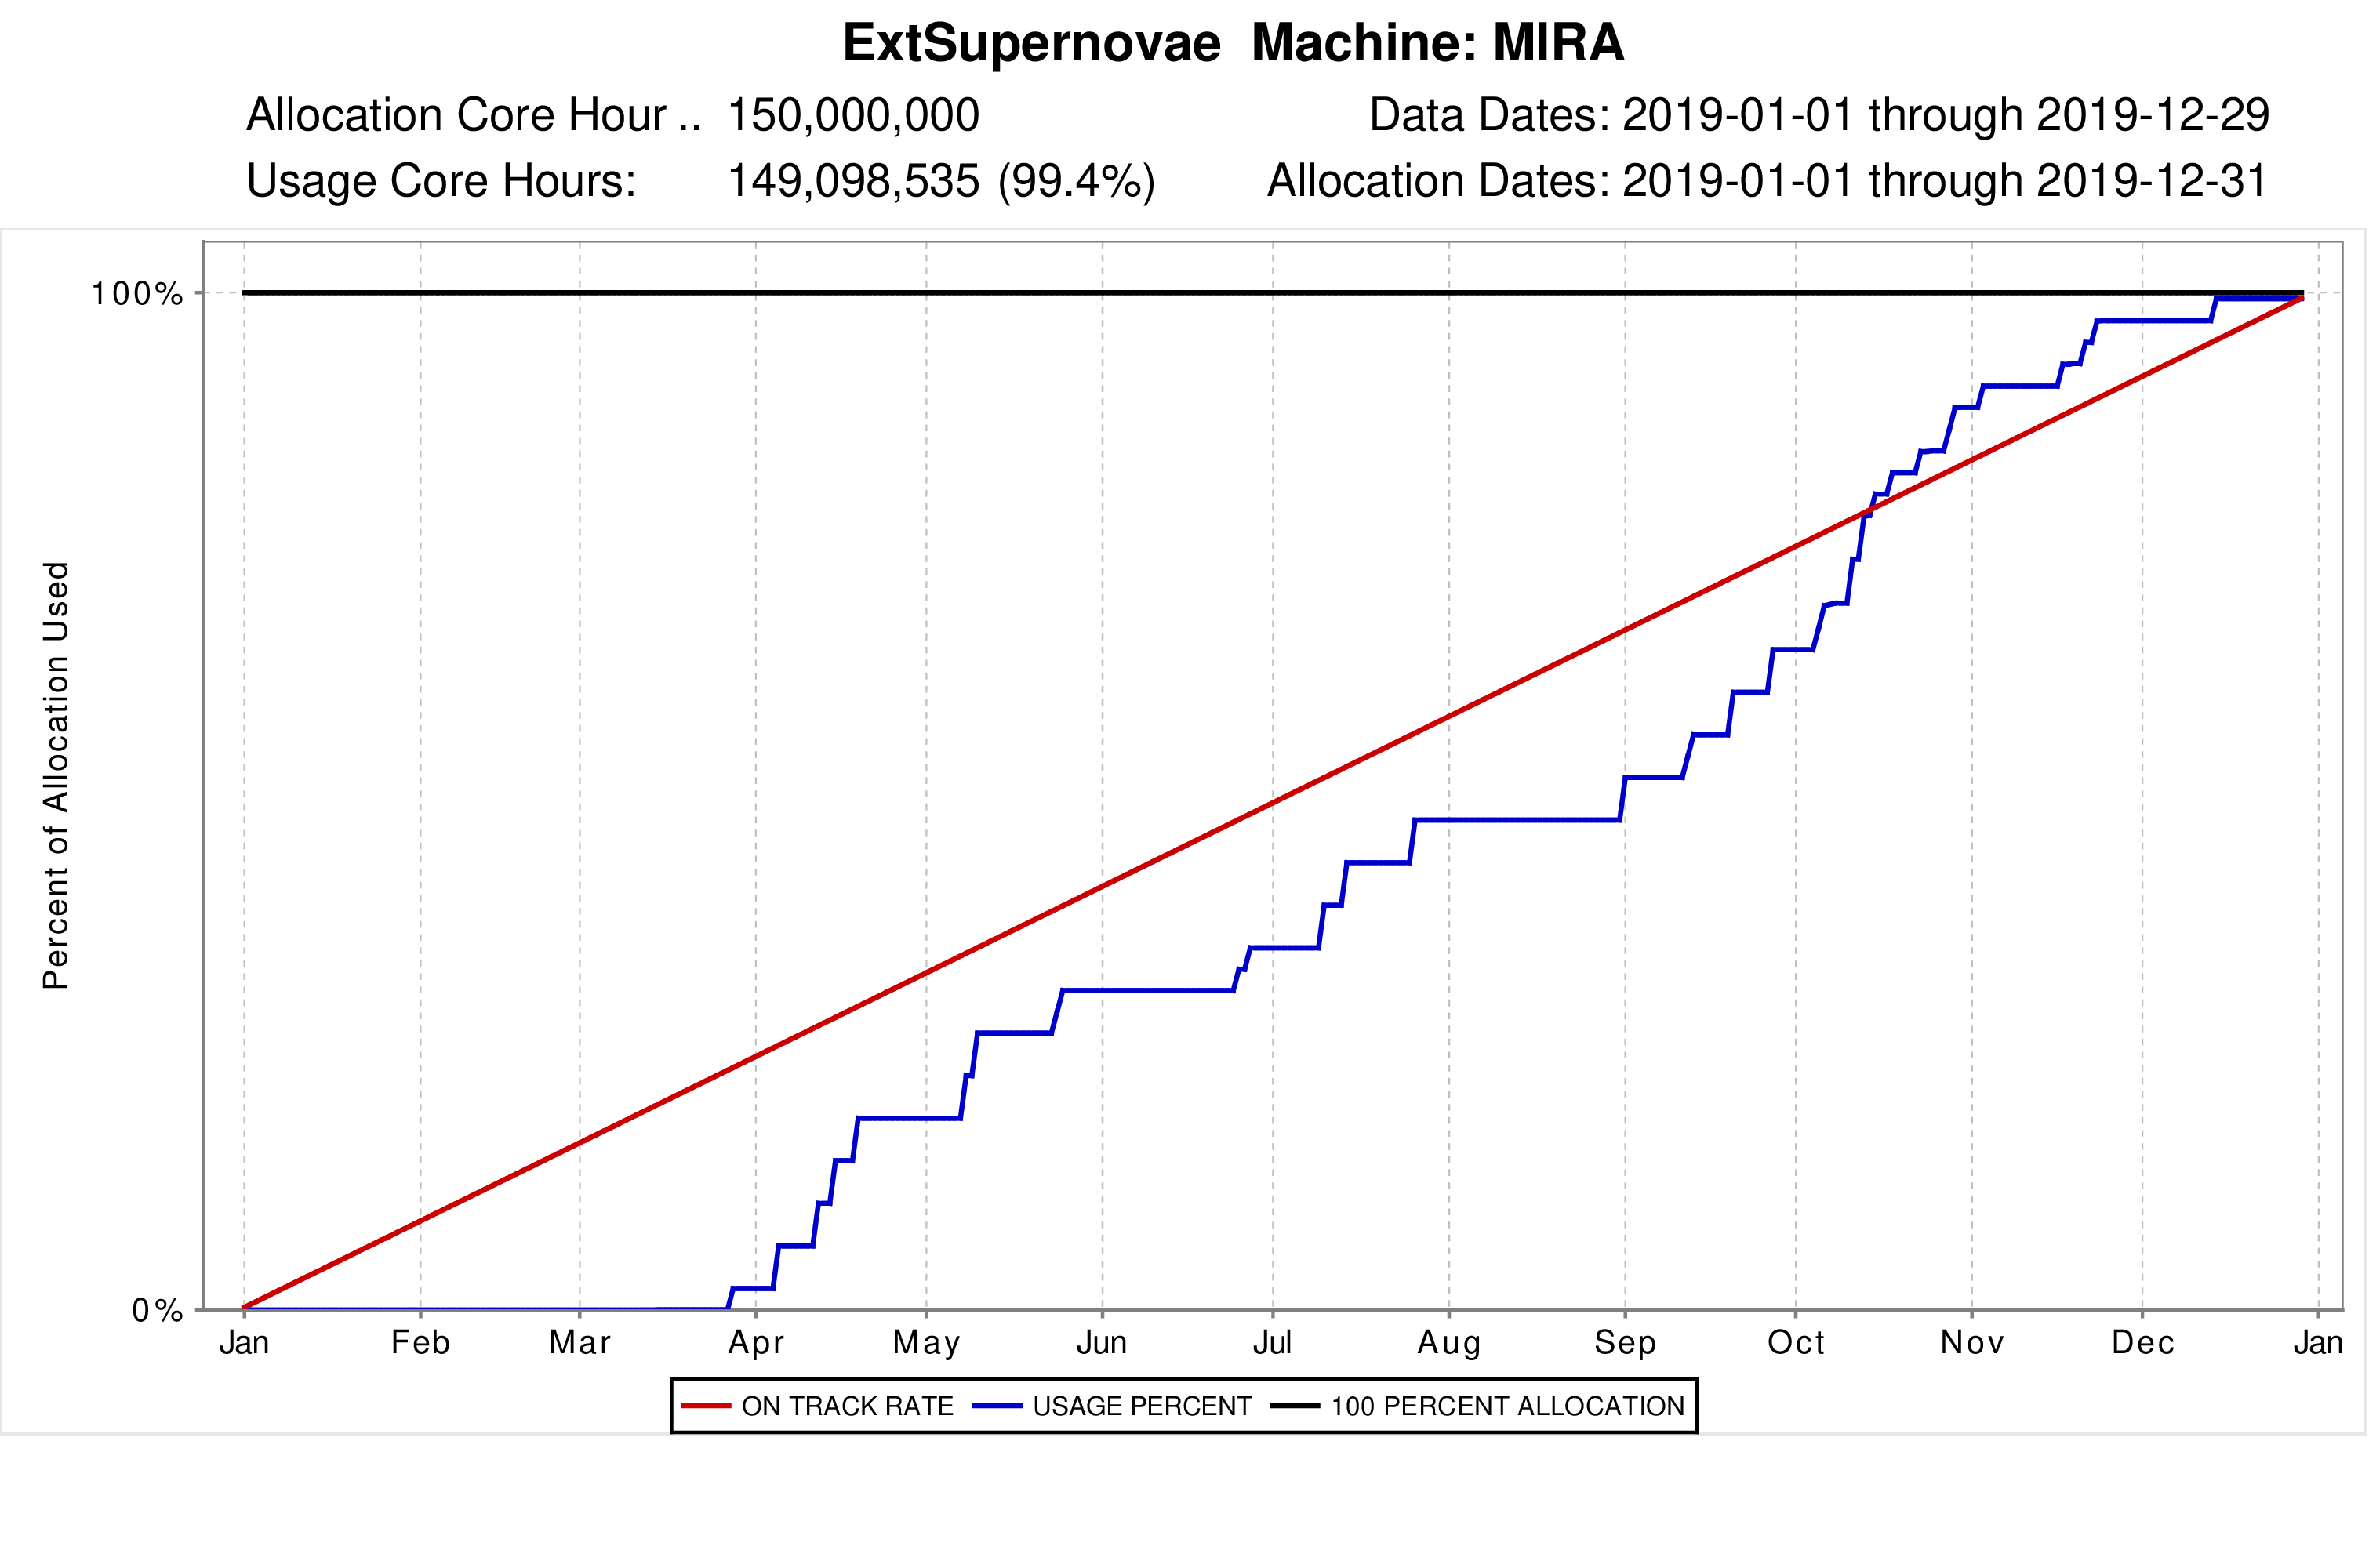
\includegraphics[width=3.25in]{on_track_graph_mira.png}
    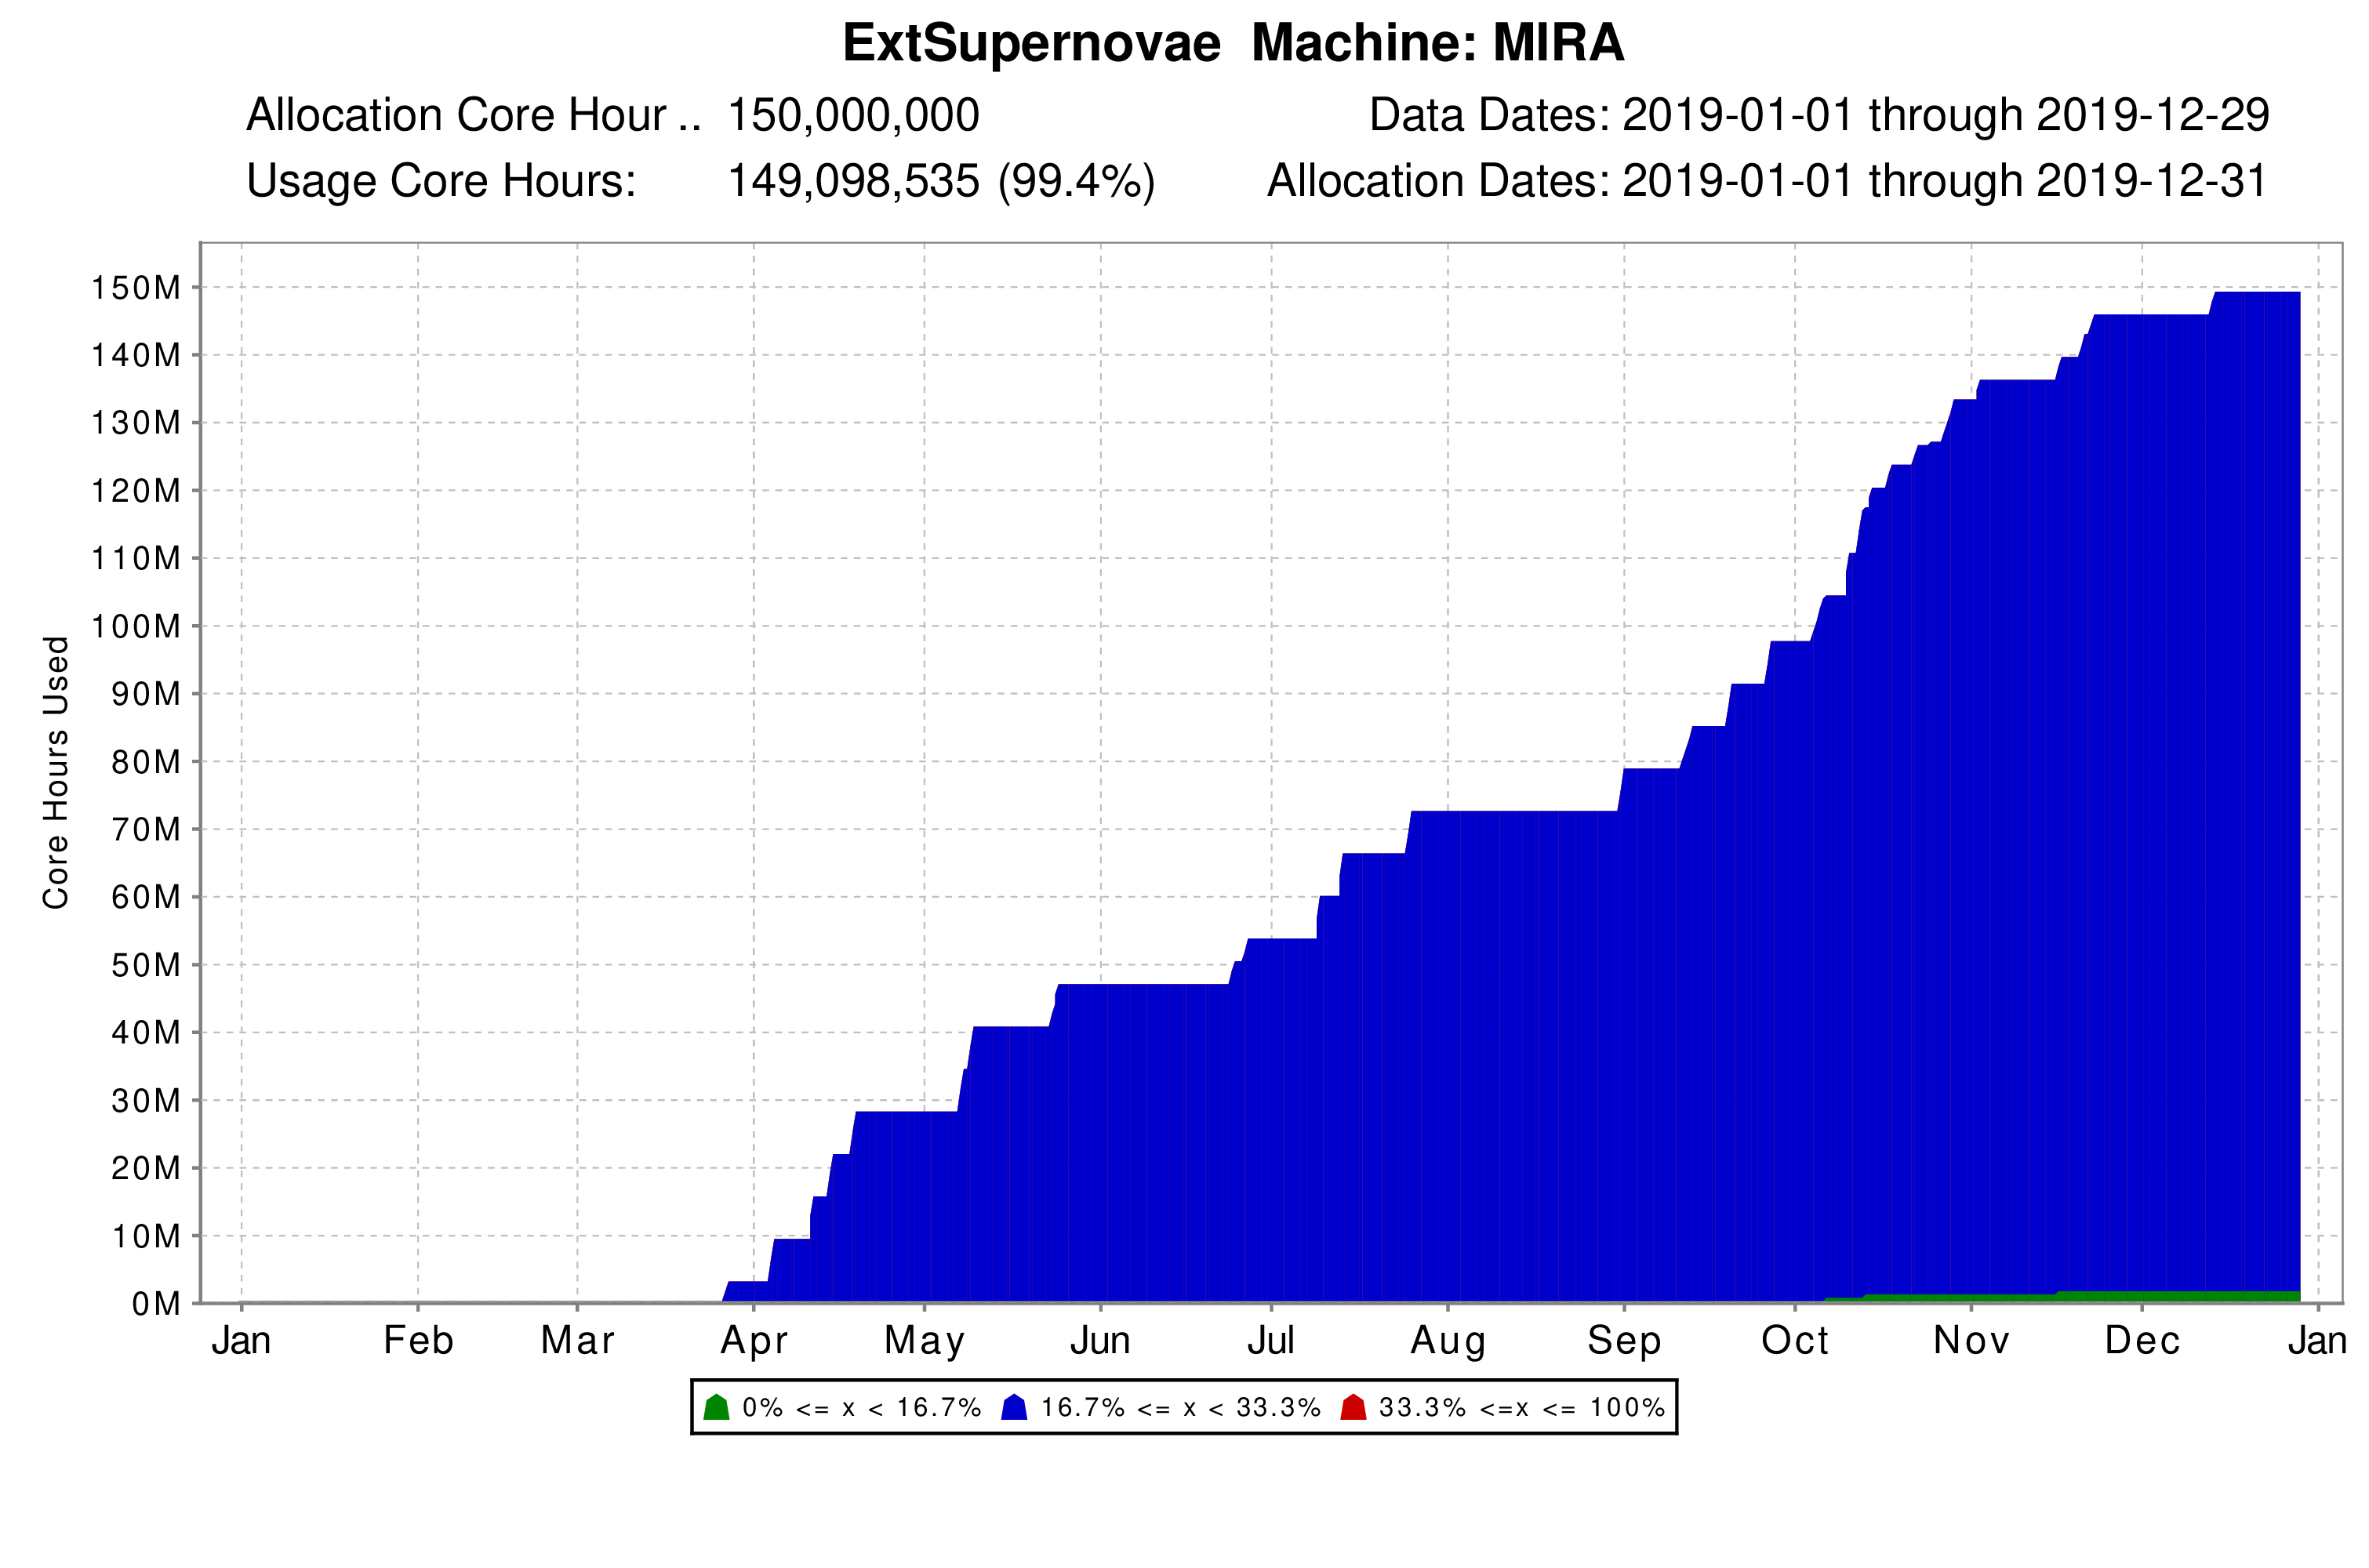
\includegraphics[width=3.25in]{categorized_hours_graph_mira.png} \\
    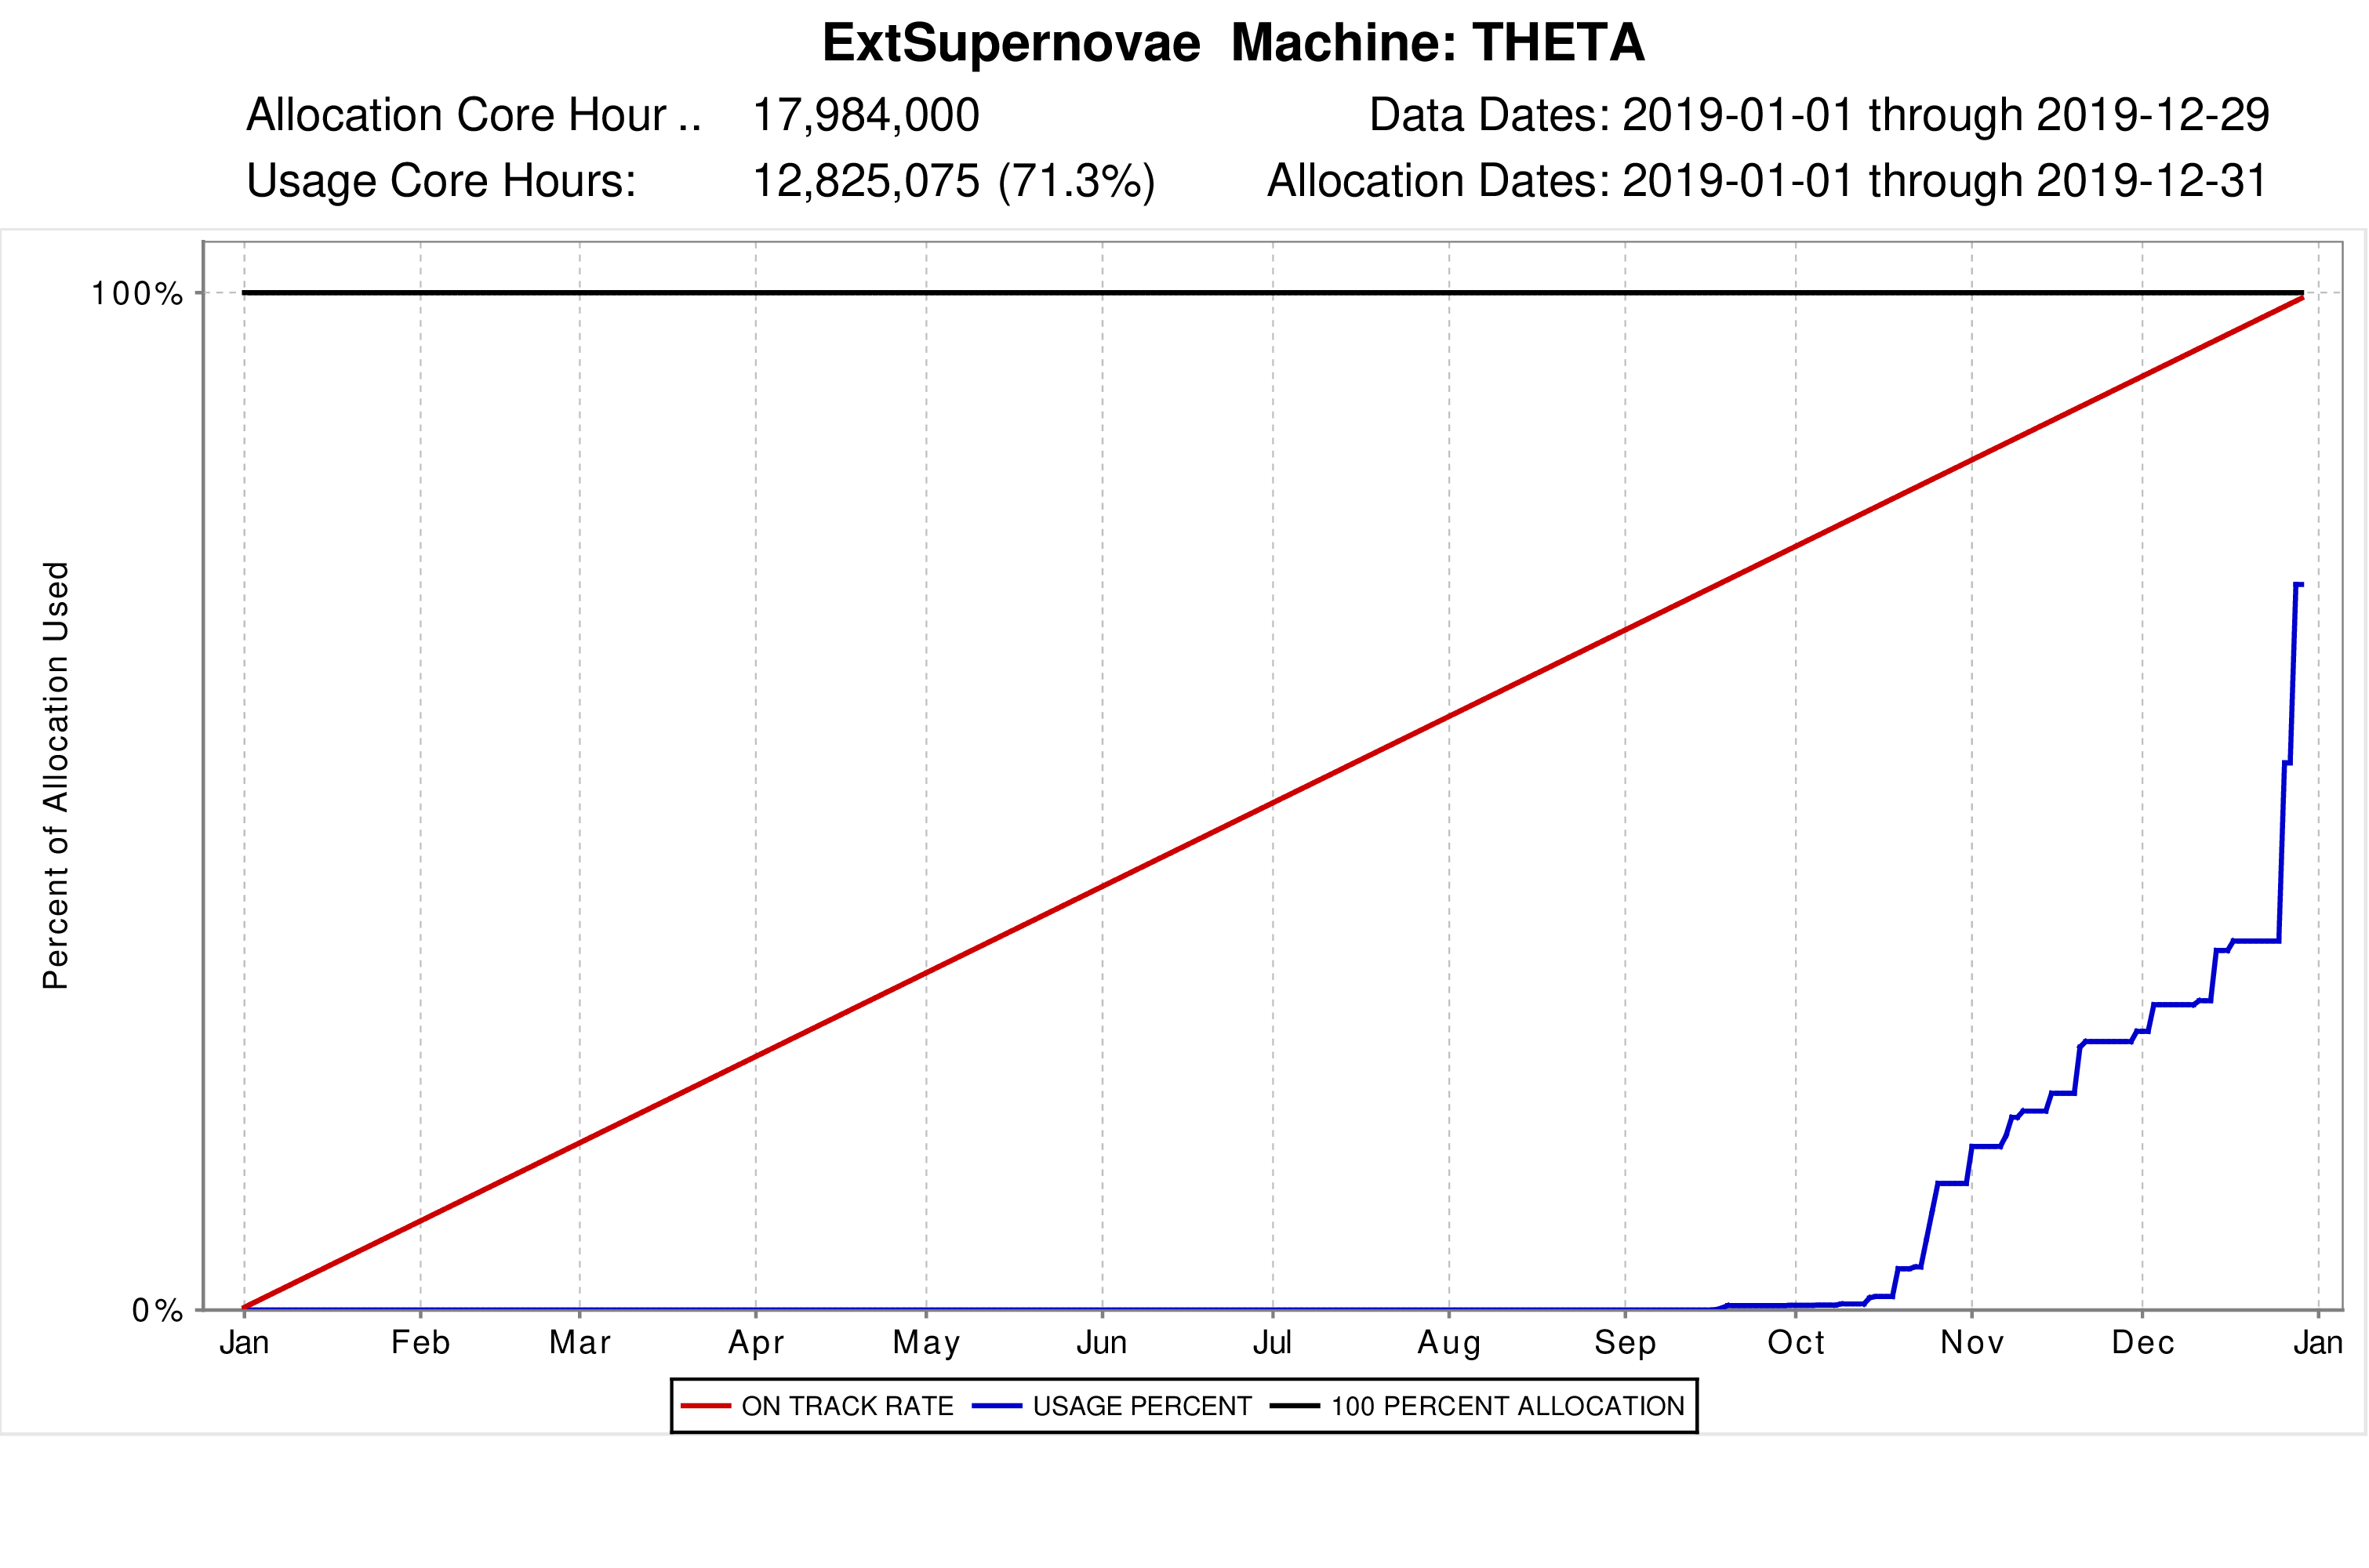
\includegraphics[width=3.25in]{on_track_graph}
    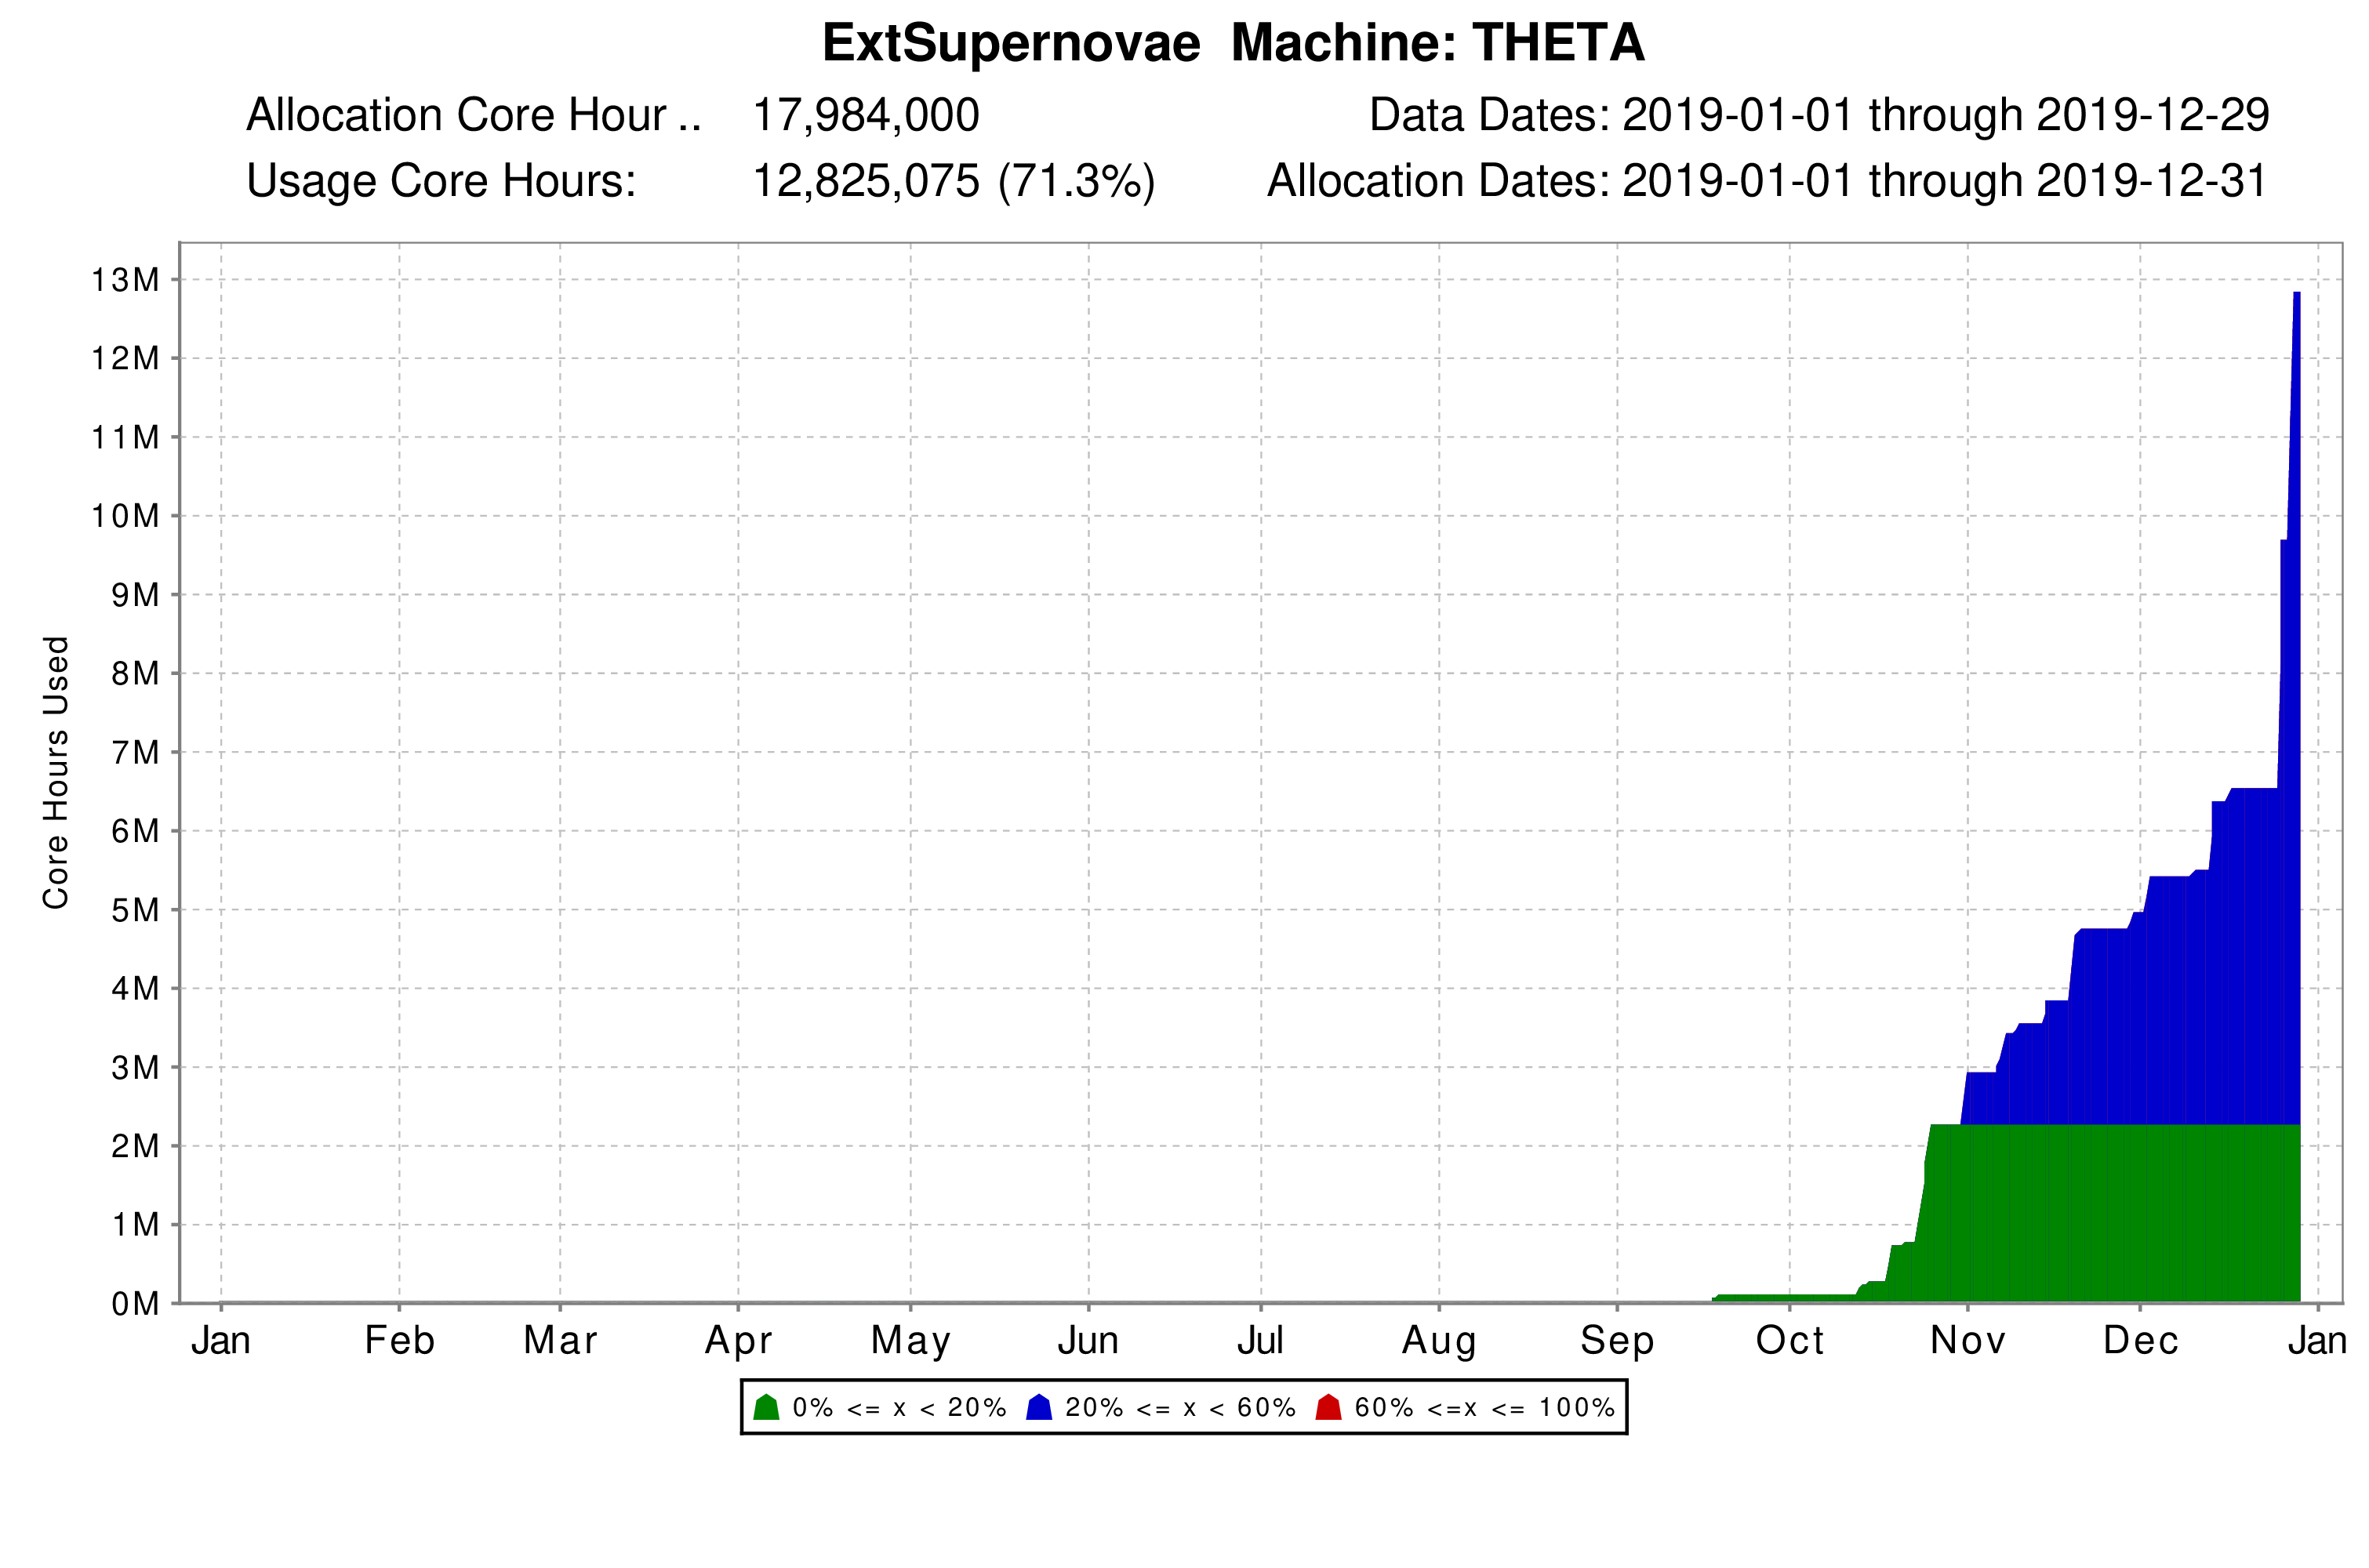
\includegraphics[width=3.25in]{categorized_hours_graph} 
  \end{tabular}
  \caption{Allocation usage.}
  \label{fig:usage}
\end{figure}

In 2019 we expended 149.1M core-hours on Mira out of our total 2019 allocation of 150M core-hours (99.4\% usage). 
Over the course of the year, we largely maintained a linear usage rate.
Longer queuing times at the very end of the year slowed us down such that we did not expend quite our full allocation, but came quite close.
Figure \ref{fig:usage} shows usage and categorized hours on Mira.
Nearly all of our usage on Mira was at the Capability scale.

After completely code tuning, and overcoming an issues with constructing a new set of initial conditions, we began production simulations on Theta in Q3. 
This put us significantly behind the linear usage rate.
We worked hard to overcome this and made tremendous progress during Q4.
We expended 12.8M core-hours on Theta out of our total 2019 allocation of 17.9M core-hours (71.3\% usage). 
This rapid progress allowed us to largely achieve our planned 2019 milestones for Theta and we are in excellent shape to make progress in 2020.
83\% of our usage on Theta was at the Capability scale.

%%%%%%%%%%%%%%%%%%%%%%%%%%%%%%%%%
\section{Report on Project Milestones}
%%%%%%%%%%%%%%%%%%%

Our milestones for Year 2, and corresponding progress, were:
\begin{enumerate}
    \item Long time simulations of MHD CCSNe - These simulations were restarted from simulations carried over from 2018 and ran in the Capability queue. Substantial progress was made on these simulations in 2019 and they are now complete.
    \item High-resolution simulation of MHD dynamos in the proto-neutron star - So far in Q1/Q2 we have analyzed simulations from 2018 that will serves as the initial conditions for this high-resolution simulation. We started this simulation in Q3. Given the extreme resolution of this simulation, it ran in the Capability queue from the outset. The target goals for this simulation were largely achieved and analysis is underway now.
    \item MHD simulation of CCSN progenitors - These simulations were deferred until 2020.
    \item CCSN simulation with 3D progenitors - This simulation ran at Capability scale on Theta. We made substantial progress on this simulation but our delays on Theta mean that we must continue this simulation in 2020.
    \item Implement microphysics from TEAMS SciDAC collaboration and neutrino-electron scattering (NES) - the TEAMS microphysics package is not yet ready for production simulations. During Q1, we finished an implementation of NES and are now using it in production on Theta.
\end{enumerate}



%%%%%%%%%%%%%%%%%%%%%%%%%%%%%%%%%
\section{Project Productivity}
%%%%%%%%%%%%%%%%%%%

\subsection{Primary}

\noindent {\bf Publications}
\begin{itemize}
    \item \href{https://ui.adsabs.harvard.edu/abs/2019arXiv191203328W}{``Constraining properties of the next nearby core-collapse supernova with multi-messenger signals''}, {Warren}, M.L., {Couch}, S.M., {O'Connor}, E.P. and {Morozova}, V, submitted to {\itshape Astrophysical Journal}, arXiv:1912.03328
    \item \href{https://ui.adsabs.harvard.edu/#abs/2019arXiv190201340C/abstract}{``Simulating Turbulence-aided Neutrino-driven Core-collapse Supernova Explosions in One Dimension''}, Couch, S. M., Warren, M. L., O'Connor, E. P. 2020, {\itshape Astrophysical Journal}, in press 
    \item \href{https://ui.adsabs.harvard.edu/#abs/2019arXiv190109055P/abstract}{``Features of Accretion Phase Gravitational Wave Emission from Two-dimensional Rotating Core-Collapse Supernovae''}, Pajkos, M. A., Couch, S. M., Pan, K., O'Connor, E. P. 2019, {\itshape Astrophysical Journal}, 878, 13
\end{itemize}

\noindent {\bf Presentations}

\begin{itemize}
    \item  ``Predictive Simulation of Multimessenger Signals from Core-collapse Supernovae ,'' S.M. Couch, PAX Multimessenger Astronomy Workshop, Penn State, February 2019
    \item ``The Turbulent Frontier in Massive Stellar Death,'' S.M. Couch, Midwest Workshop on Supernovae and Transients, February 2019
    \item ``Gravitational Waves from Core-collapse Supernovae,'' S.M. Couch, LIGO SN Group Seminar, March 2019
    \item ``Multidimensionl Supernova Progenitors,'' S.M. Couch, SciDAC TEAMS Collaboration Meeting, May 2019
    \item ``Predicting Supernova Neutrino Signals,'' M. Warren, Supernova Early Warning System (SNEWS) 2.0 Workshop, June 2019
    \item ``High-order MHD for Supernovae,'' S.M. Couch, ASTRONUM 2019, July 2019
    \item ``Toward a Predictive Theory of Core-collapse Supernova Explosions,'' S.M. Couch, Wayne State University Particle Astrophysics Seminar, October 2019.
\end{itemize}

% \subsubsection{Secondary}

% \begin{itemize}
%   \item Co-I and postdoc Kuo-Chuan Pan started a tenure-track faculty position at National Tsing Hua University in Taiwan.
%   \item Co-I and postdoc MacKenzie Warren won a prestigious NSF Postdoctoral Fellowship.
% \end{itemize}

\section{Center Feedback}

Our catalyst, Adrian Pope, has been extremely helpful.
He is now helping us tune our code for Theta.


\section{Code Description and Characterization}

\texttt{FLASH} is a highly capable, fully modular, extensible,
community code that is widely used in astrophysics, cosmology, fluid
dynamics, and plasma physics, and other fields.  The capabilities of
the FLASH code include adaptive mesh refinement (AMR), several
self-gravity solvers, an advection-diffusion-reaction (ADR) flame
model, an accurate and detailed treatment of nuclear burning, and a
sophisticated two-moment neutrino transport scheme based on an
explicit hyperbolic solver.  The neutrino interactions are included
through the open-source neutrino interaction library
\texttt{NuLib}. We have enhanced the
performance of the two-moment neutrino transport scheme significantly
as well as upgraded the transport to now include full velocity and
gravitational red-shift dependence in the evolution equations.

\texttt{FLASH} is written in modern Fortran, with some utility
functions written in C, and a build system written in Python.  It
requires MPI library support, and either HDF5 or P-NetCDF for I/O.
Additional mathematical software, such as \texttt{Hypre}, may be
required to configure \texttt{FLASH} for particular simulations.

Algorithm classes used within \texttt{FLASH} include Sparse Linear
Algebra solvers, FFT, active and passive particles, structured grids,
and AMR.



\end{document}
